\documentclass[12pt,a4paper]{article}

\usepackage[utf8]{inputenc}
\usepackage[T1]{fontenc}
\usepackage[spanish]{babel}
\usepackage{graphicx}
\usepackage{geometry}
\usepackage{hyperref}
\usepackage{float}
\usepackage{caption}
\usepackage{array}
\usepackage{tabularx}
\usepackage{tikz}
\usetikzlibrary{arrows.meta,positioning,shapes.geometric,shapes.multipart,calc}

\geometry{top=1.5cm,bottom=1.5cm,left=1.8cm,right=1.8cm}
\hypersetup{colorlinks=true,urlcolor=blue}
\setlength{\parindent}{0pt}
\renewcommand{\arraystretch}{1.18}
\newcolumntype{Y}{>{\centering\arraybackslash}X}

% Estilos TikZ usados para reproducir los diagramas realizados manualmente.
\tikzset{
  umlclass/.style={
    rectangle split,
    rectangle split parts=3,
    rectangle split draw splits=true,
    draw,
    minimum width=4.2cm,
    text width=4.0cm,
    align=left,
    inner sep=2mm,
    font=\small
  },
  activity/.style={
    draw,
    rectangle,
    minimum width=3.6cm,
    minimum height=1.0cm,
    align=center,
    font=\small
  },
  decision/.style={
    diamond,
    draw,
    aspect=1.35,
    minimum width=2.4cm,
    minimum height=1.45cm,
    align=center,
    inner sep=1pt,
    font=\small
  },
  flow/.style={-{Latex[length=2.5mm]},thick},
  statefinal/.style={circle,draw,double,minimum size=6mm,inner sep=0pt}
}

\begin{document}
\thispagestyle{empty}

\begin{center}
{\large\textbf{UNIVERSIDAD TÉCNICA ESTATAL DE QUEVEDO}}\\
{\normalsize FACULTAD DE CIENCIAS DE LA COMPUTACIÓN}\\
{\normalsize CARRERA DE INGENIERÍA DE SOFTWARE -- 4TO NIVEL}\\[0.3cm]
\rule{\textwidth}{0.5pt}\\[0.25cm]

{\Large\textbf{PRUEBA PRÁCTICA -- UNIDAD IV}}\\
{\normalsize Validación, Gestión, Herramientas y Estándares de Requisitos}\\
{\normalsize Caso: Sistema de Gestión de Pedidos}\\[0.25cm]
\rule{\textwidth}{0.5pt}\\[0.3cm]

\begin{tabular}{rl}
\textbf{Asignatura:} & Ingeniería de Requerimientos \\
\textbf{Estudiante:} & Mora Duarte Alex José \\
\textbf{Docente:} & Ing. Gleiston Guerrero, Mg. \\
\textbf{Fecha:} & 11/08/2026 \\
\end{tabular}\\[0.25cm]

\textbf{Repositorio:}\\[-0.05cm]
\url{https://github.com/amorad35/Mora-IRS401-Prueba_U4.git}\\[0.3cm]

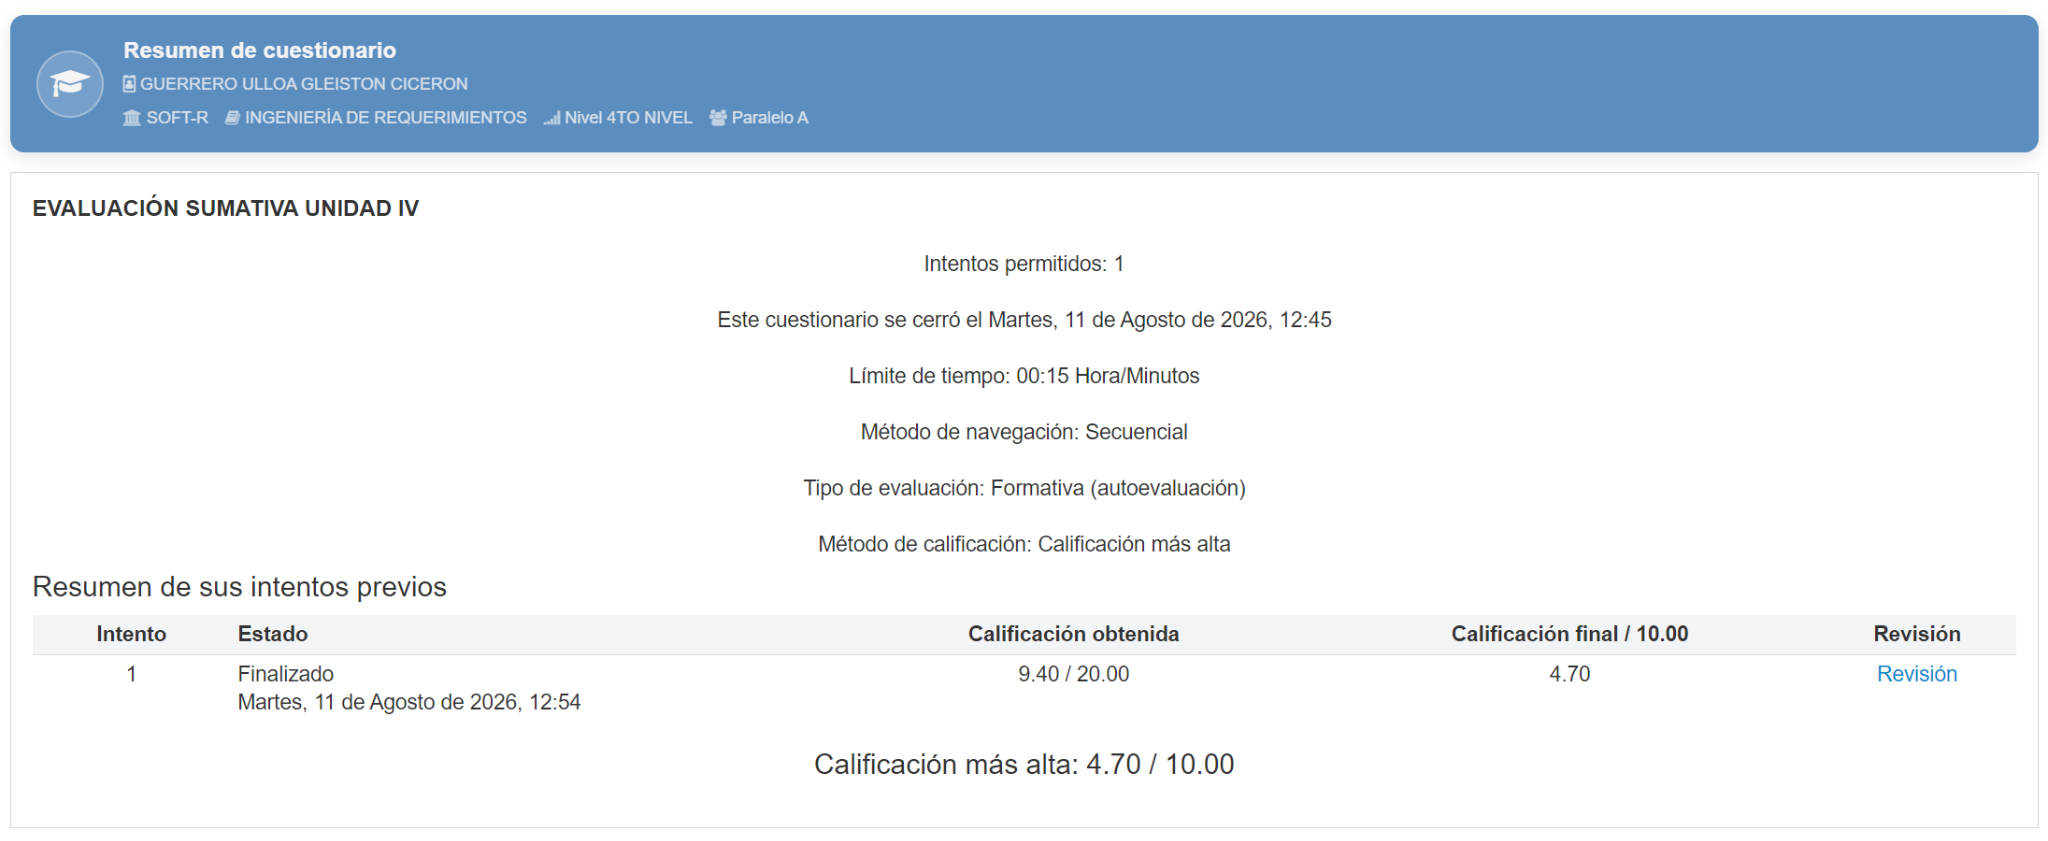
\includegraphics[width=0.95\textwidth]{figuras/01_resumen_cuestionario_sga.png}\\[-0.05cm]
{\small\textit{Figura 1. Resumen del cuestionario en el SGA.}}\\[0.25cm]

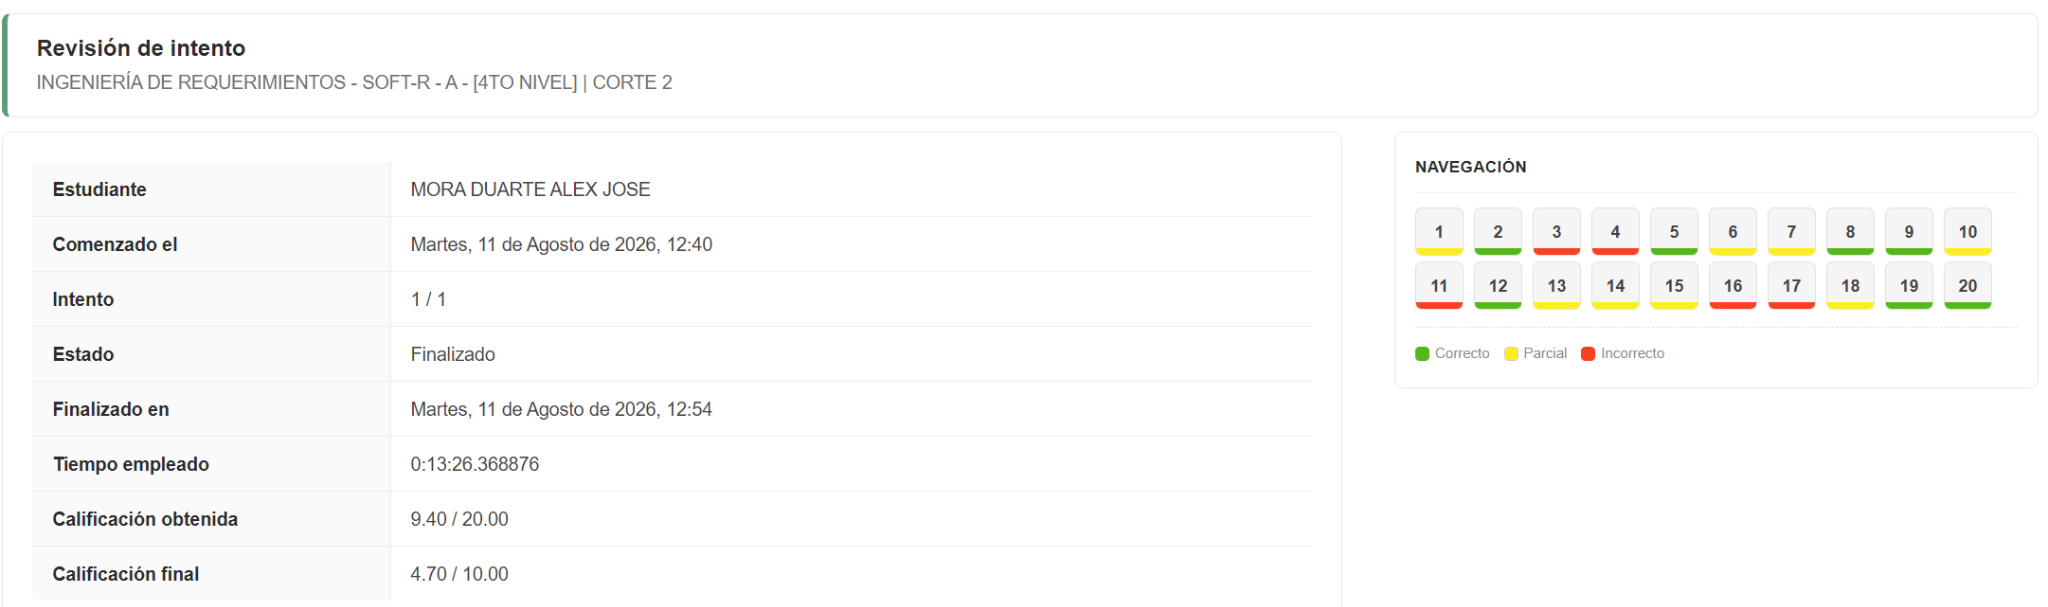
\includegraphics[width=0.95\textwidth]{figuras/02_evaluacion_intento_sga.png}\\[-0.05cm]
{\small\textit{Figura 2. Evaluación/revisión del intento en el SGA.}}\\[0.25cm]

\vfill
Quevedo -- Ecuador\\
2026
\end{center}

\clearpage
\setcounter{page}{1}
\pagestyle{plain}

% ============================================================
% P1 - Transcripción gráfica de lo realizado manualmente
% ============================================================
\section*{P1. Modelo de datos -- Diagrama de clases UML}

\begin{center}
\resizebox{\textwidth}{!}{%
\begin{tikzpicture}[node distance=2.4cm and 2.5cm]

\node[umlclass] (cliente) {
  \nodepart{one}\centering\textbf{Cliente}
  \nodepart{two}
  idDocumento : integer\\
  nombreCliente : string\\
  correoCliente : string
  \nodepart{three}
  +realizarPedido()
};

\node[umlclass, right=2.4cm of cliente] (pedido) {
  \nodepart{one}\centering\textbf{Pedido}
  \nodepart{two}
  idPedido : integer\\
  fecha : date\\
  total : decimal\\
  estado : string
  \nodepart{three}
  +calcularTotal()\\
  +confirmar()
};

\node[umlclass, right=2.4cm of pedido] (linea) {
  \nodepart{one}\centering\textbf{LineaPedido}
  \nodepart{two}
  idLinea : integer\\
  cantidad : integer\\
  subtotal : decimal
  \nodepart{three}
  +calcularSubtotal()
};

\node[umlclass, below=2.7cm of linea] (producto) {
  \nodepart{one}\centering\textbf{Producto}
  \nodepart{two}
  idProducto : integer\\
  descripcion : string\\
  precio : decimal\\
  stock : integer
  \nodepart{three}
  +verificarStock()
};

% Cliente - Pedido
\draw (cliente.east) -- (pedido.west)
  node[midway,below=2pt]{\small realiza};
\node[above right=0pt and 2pt of cliente.east]{\small 1};
\node[above left=0pt and 2pt of pedido.west]{\small 0..*};

% Pedido - LineaPedido
\draw (pedido.east) -- (linea.west)
  node[midway,below=2pt]{\small contiene};
\node[above right=0pt and 2pt of pedido.east]{\small 1};
\node[above left=0pt and 2pt of linea.west]{\small 1..*};

% LineaPedido - Producto
\draw (linea.south) -- (producto.north)
  node[midway,right=4pt]{\small referencia};
\node[below right=2pt and 2pt of linea.south]{\small 0..*};
\node[above right=2pt and 2pt of producto.north]{\small 1};

\end{tikzpicture}%
}
\end{center}

% ============================================================
% P2 - Reproducción fiel del diagrama realizado manualmente
% ============================================================
\section*{P2. Modelo funcional -- Diagrama de actividades UML}

\begin{center}
\begin{tikzpicture}[x=1cm,y=1cm]

% Carriles Usuario / Sistema
\draw (-5.2,7.9) rectangle (5.2,-4.75);
\draw (0,7.9) -- (0,-4.75);
\draw (-5.2,7.1) -- (5.2,7.1);
\node at (-2.6,7.5) {\textbf{Usuario}};
\node at (2.6,7.5) {\textbf{Sistema}};

% Inicio en el carril Usuario
\fill (-2.6,6.55) circle (2.2pt);
\node[above=2pt] at (-2.6,6.55) {\small Inicio};

% Actividades superiores
\node[activity, minimum width=4.1cm] (clienteA) at (-2.6,5.45)
  {Registrar datos de\\cliente};
\node[activity, minimum width=4.1cm] (productoA) at (-2.6,3.65)
  {Registrar datos de\\Producto};
\node[activity, minimum width=4.35cm] (stockA) at (2.55,3.65)
  {Verificar disponibilidad\\de stock};
\node[decision, aspect=1.55, minimum width=2.65cm, minimum height=1.5cm]
  (stockD) at (2.55,1.75) {¿Hay\\stock?};

% Registrar pedido permanece completamente en el carril Sistema
\node[activity, minimum width=2.15cm] (registrarA) at (1.15,-0.05)
  {Registrar\\Pedido};

% Acciones finales en el carril Usuario, como en el dibujo manual
\node[activity, minimum width=2.2cm] (confirmarA) at (-3.75,-2.05)
  {Confirmar\\Pedido};
\node[activity, minimum width=2.35cm] (faltanteA) at (-1.25,-2.05)
  {Notificar\\Faltante};

% Flujo principal
\draw[flow] (-2.6,6.52) -- (clienteA.north);
\draw[flow] (clienteA.south) -- (productoA.north);
\draw[flow] (productoA.east) -- (stockA.west);
\draw[flow] (stockA.south) -- (stockD.north);

% Rama Sí -> Registrar pedido -> Confirmar pedido
% La salida Sí baja a Registrar Pedido dentro del carril Sistema.
\draw[flow] (stockD.west) -- (1.15,1.75)
  node[midway,above]{\small Sí}
  -- (1.15,0.70) -- (registrarA.north);

% Desde Registrar Pedido la flecha sale por la izquierda,
% recorre horizontalmente hasta la vertical de Confirmar Pedido
% y baja directamente hacia Confirmar Pedido.
\draw[flow] (registrarA.west) -- (-3.75,-0.05) -- (confirmarA.north);

% Rama No -> Notificar faltante
% Sale por la derecha del rombo y termina en Notificar Faltante.
\draw[flow] (stockD.east) -- (4.15,1.75)
  node[midway,above]{\small No}
  -- (4.15,-1.15) -- (-1.25,-1.15) -- (faltanteA.north);

% Unión inferior: una sola línea recta, como en la hoja
\coordinate (unionL) at (-3.75,-3.05);
\coordinate (unionR) at (-1.25,-3.05);
\coordinate (unionM) at (-2.50,-3.05);

\draw (confirmarA.south) -- (unionL);
\draw (faltanteA.south) -- (unionR);
\draw (unionL) -- (unionR);
\fill (unionM) circle (1.7pt);

% Desde el punto de unión sale directamente hacia el fin
\node[statefinal] (finP) at (-2.50,-3.82) {};
\draw[flow] (unionM) -- (finP.north);
\node[below=1pt of finP] {\small Fin};

\end{tikzpicture}
\end{center}

% ============================================================
% P3 - Se conserva la forma vertical realizada manualmente.
% ============================================================
\section*{P3. Modelo de comportamiento -- Máquina de estados UML}

\begin{center}
\begin{tikzpicture}[node distance=1.35cm]
\fill (0,0) circle (2.4pt);

\node[below=0.9cm of {(0,0)}, align=center] (r1) {registrar [Registrado]};
\node[below=1.15cm of r1, align=center] (r2) {confirmar [stock disponible] [Confirmar]};
\node[below=1.15cm of r2, align=center] (r3) {despachar [Enviado]};
\node[below=1.15cm of r3, align=center] (r4) {entregar [Entregado]};
\node[statefinal, below=0.9cm of r4] (rfin) {};

\draw[flow] (0,-0.08) -- (r1.north);
\draw[flow] (r1.south) -- (r2.north);
\draw[flow] (r2.south) -- (r3.north);
\draw[flow] (r3.south) -- (r4.north);
\draw[flow] (r4.south) -- (rfin.north);
\end{tikzpicture}
\end{center}

% ============================================================
% P4 - Contenido transcrito de la tabla manual.
% ============================================================
\section*{P4. Consistencia entre las tres perspectivas}

\begin{center}
\small
\setlength{\tabcolsep}{5pt}
\begin{tabularx}{0.96\textwidth}{|>{\raggedright\arraybackslash}p{2.2cm}|>{\raggedright\arraybackslash}X|>{\raggedright\arraybackslash}p{4.0cm}|}
\hline
\textbf{Evento} & \textbf{Acción} & \textbf{Afectado} \\
\hline
registrar & Crear/registrar pedido & idPedido, fecha, total \\
\hline
confirmar & Confirmar pedido & estado \\
\hline
despachar & no aparece inicialmente & estado \\
\hline
entregar & no aparece inicialmente & estado \\
\hline
anular & no aparece inicialmente & estado \\
\hline
\end{tabularx}
\end{center}

% ============================================================
% P5 - Solo se incorpora lo escrito manualmente.
% ============================================================
\section*{P5. Especificación de requisitos con esquema de atributos}
\vspace{-0.15cm}

\textbf{RF-1 Registrar Pedido}

\begin{center}
\small
\setlength{\tabcolsep}{3.6pt}
\renewcommand{\arraystretch}{1.08}
\begin{tabularx}{0.98\textwidth}{|c|c|c|Y|c|c|Y|}
\hline
\textbf{ID} & \textbf{Prioridad} & \textbf{Estado} & \textbf{Fuente} & \textbf{Estabilidad} & \textbf{Versión} & \textbf{Verificación} \\
\hline
RF-1 & Must & Propuesto & Caso Práctico & Alta & 1.0 & Prueba funcional \\
\hline
\end{tabularx}
\end{center}

\textbf{RF-2 Anular Pedido}

\begin{center}
\small
\setlength{\tabcolsep}{3.6pt}
\renewcommand{\arraystretch}{1.08}
\begin{tabularx}{0.98\textwidth}{|c|c|c|Y|c|c|Y|}
\hline
\textbf{ID} & \textbf{Prioridad} & \textbf{Estado} & \textbf{Fuente} & \textbf{Estabilidad} & \textbf{Versión} & \textbf{Verificación} \\
\hline
RF-2 & Should & Propuesto & Caso práctico & Alta & 1.0 & Prueba funcional \\
\hline
\end{tabularx}
\end{center}

\textbf{RNF-1 Eficiencia de desempeño}

\begin{center}
\small
\setlength{\tabcolsep}{3.6pt}
\renewcommand{\arraystretch}{1.08}
\begin{tabularx}{0.98\textwidth}{|c|c|c|Y|c|c|Y|}
\hline
\textbf{ID} & \textbf{Prioridad} & \textbf{Estado} & \textbf{Fuente} & \textbf{Estabilidad} & \textbf{Versión} & \textbf{Verificación} \\
\hline
RNF-1 & Must & Propuesto & Caso práctico & Alta & 1.0 & Prueba funcional \\
\hline
\end{tabularx}
\end{center}

\textbf{RNF-2 Seguridad}

\begin{center}
\small
\setlength{\tabcolsep}{3.6pt}
\renewcommand{\arraystretch}{1.08}
\begin{tabularx}{0.98\textwidth}{|c|c|c|Y|c|c|Y|}
\hline
\textbf{ID} & \textbf{Prioridad} & \textbf{Estado} & \textbf{Fuente} & \textbf{Estabilidad} & \textbf{Versión} & \textbf{Verificación} \\
\hline
RNF-2 & Must & Propuesto & Caso práctico & Alta & 1.0 & Prueba funcional \\
\hline
\end{tabularx}
\end{center}
\normalsize

% ============================================================
% P6 - Contenido transcrito de la tabla manual.
% ============================================================
\section*{P6. Priorización MoSCoW}

\begin{center}
\small
\setlength{\tabcolsep}{5pt}
\begin{tabularx}{0.96\textwidth}{|c|c|X|}
\hline
\textbf{Requisito} & \textbf{Prioridad} & \textbf{Justificación} \\
\hline
RF-1 & Must & Es la función principal del sistema. \\
\hline
RF-2 & Should & Es importante en caso de rechazar o anular pedido. \\
\hline
RNF-1 & Must & El caso exige registrar con rapidez. \\
\hline
RNF-2 & Must & El caso exige proteger datos personales. \\
\hline
\end{tabularx}
\end{center}

% ============================================================
% P7 - Contenido transcrito de la lista de comprobación manual.
% ============================================================
\section*{P7. Validación por inspección}

\begin{center}
\small
\setlength{\tabcolsep}{3.5pt}
\begin{tabularx}{0.94\textwidth}{|c|Y|Y|Y|Y|Y|}
\hline
\textbf{Requisito} & \textbf{No ambiguo} & \textbf{Completo} & \textbf{Singular} & \textbf{Verificable} & \textbf{Factible} \\
\hline
RF-1 & Sí & Sí & Sí & Sí & Sí \\
\hline
RF-2 & Sí & No & Sí & Sí & Sí \\
\hline
RNF-1 & No & Sí & Sí & Sí & Sí \\
\hline
RNF-2 & Sí & Sí & Sí & Sí & Sí \\
\hline
\end{tabularx}
\end{center}

\end{document}
